\chapter{Υλοποίηση συστήματος Procedural Content Generation}

Την υλοποίηση αυτής της εργασίας μπορούμε να την χωρίσουμε σε δύο ξεχωριστά εννοιολογικά κομμάτια. Το πρώτο κομμάτι αφορά την υλοποίηση ενός \textit{Procedural Content Generation} συστήματος όπως αυτά που περιγράψαμε στο προηγούμενο κεφάλαιο, και σε ένα \textit{Machine Learning Content Generation} σύστημα. Σε αυτό το κεφάλαιο αναλύουμε την τεχνική υλοποίηση του PCG.
\par
Από το στάδιο της αρχικής ιδέας μέχρι την έναρξη της υλοποίησης μπορούμε να διακρίνουμε ένα ενδιάμεσο στάδιο, του σχεδιασμού και της έρευνας σχετικά με τις τεχνολογίες, τις δομές δεδομένων και τους αλγορίθμους που θα κληθούμε να υλοποιήσουμε. Αυτή η ιεραρχία από την ιδέα έως την υλοποίηση, ισχύει για όλες τις εφαρμογές της επιστήμης της πληροφορικής και ειδικότερα του game development \textit{gamedevprocess}, όπου έχουμε πολλά υποσυστήματα που θα πρέπει να λειτουργήσουν παράλληλα και να συνεργαστούν με το σύστημα του PCG. Η σωστή οργάνωση και σχεδίαση της αρχιτεκτονικής του PCG είναι ένα πολύ κρίσιμο κομμάτι.
\par
Κατά την υλοποίηση και ιδιαίτερα κατά το στάδιο της αξιολόγησης όπως είδαμε μπορεί να προκύψουν προβλήματα όπως μη αποδεκτά αποτελέσματα, γεγονός που μπορεί να οδηγήσει στον ανασχεδιασμό και την επιλογή διαφορετικών αλγορίθμων ή παραμέτρων. Αυτή η διαδικασία μπορεί να επαναληφθεί πολλές φορές καθώς, όπως αναλύθηκε, τα \textit{καλά} συστήματα PCG βγαίνουν μέσα από δοκιμές και λάθη (\textit{trial and error}).
\par
Η υλοποίηση ενός τέτοιου συστήματος μπορεί να θεωρηθεί, και είναι και η προσωπική εμπειρία της συγγραφέας, ως μια πολύ δημιουργική εργασία, ειδικά σε σύγκριση με την διαδικασία ανάπτυξης άλλων ειδών λογισμικού. Προβλήματα που απαιτούν σκέψη \textit{outside of the box} και δημιουργικότητα, σε συνδυασμό με πολύ καλή γνώση της θεωρίας και της τεχνολογίας είναι ένα από τα χαρακτηριστικά που κάνουν αυτόν τον τομέα της πληροφορικής, τόσο ενδιαφέρον και ιδιαίτερο.

\section{Game Engines}
Τα Συστήματα Δημιουργίας Ηλεκτρονικών Παιχνιδιών (\textit{Game Engines}) είναι σχεδιαστικά περιβάλλοντα υλοποίησης παιχνιδιών, που χρησιμοποιούνται από εταιρείες και ομάδες ανθρώπων σε ολόκληρο τον κόσμο για την δημιουργία ηλεκτρονικών παιχνιδιών. Συνήθως περιλαμβάνουν συστήματα που βοηθάνε τους προγραμματιστές και σχεδιαστές, όπως το σύστημα προσομοίωσης νόμων της φυσικής, κίνησης αντικειμένων, βαρύτητα κ.ά. (Physics Engine). \cite{gameengine}
\par
Τα συστήματα που έχουν τα περισσότερα Game Engines είναι το σύστημα για την καταγραφή και επεξεργασία των εισόδων του χρήστη, όπως το πάτημα ενός κουμπιού, η κίνηση του ποντικιού κ.ά (Input Engine), σύστημα για την εμφάνιση γραφικών (\textit{textures}, \textit{sprites}) (Graphics Engine), σύστημα για την κίνηση αντικειμένων με γραφικά (\textit{animations})(Animation Engine) και πολλά ακόμη.
\par
Υπάρχουν Game Engines που εξειδικεύονται στην δημιουργία ενός συγκεκριμένου είδους παιχνιδιού, όπως για παράδειγμα το \textit{Hero Engine} εξειδικεύεται στην δημιουργία παιχνιδιών που παίζονται μέσω Internet (\textit{Online video games}). Αυτό σημαίνει ότι το Hero Engine έχει πολύ καλά ανεπτυγμένα συστήματα για την επικοινωνία \textit{client-server} εφαρμογών σε πραγματικό χρόνο καθώς και την διαχείριση δεδομένων που αποθηκεύονται κεντρικά σε κάποιο \textit{servers}.
\par
Επίσης υπάρχουν και τα Game Engines που δεν φαίνεται να έχουν κάποια εξειδίκευση, αλλά υποστηρίζουν το κάθε είδους game που θέλουμε να αναπτύξουμε. Αυτά τα Game Engine έχουν γνωρίσει μεγάλη δημοτικότητα τα τελευταία χρόνια, σε συνδυασμό με το γεγονός ότι είναι ελεύθερα διαθέσιμα, με αποτέλεσμα να διευρυνθεί η χρήση τους με μεγάλη επιτυχία από ομάδες όλων των μεγεθών (μικρά independent studio και developers μέχρι μεγάλες εταιρείες). Τέτοια Game Engines είναι το Unity Engine \cite{unity}, το Unreal Engine \cite{unreal}, το Godot Engine (το οποίο είναι OpenSource) \cite{godot} κ.ά.
\par
Η εκμάθηση ενός τέτοιου προγράμματος απαιτεί χρόνο και μελέτη, καθώς το κάθε Game Engine έχει δικές του υλοποιήσεις για το κάθε σύστημα, διαφορετικό περιβάλλον αλληλεπίδρασης με τον χρήστη (\textit{editor}) καθώς και διαφορετική γλώσσα προγραμματισμού που πρέπει να χρησιμοποιήσει ο προγραμματιστής. Υπάρχουν πολλά κριτήρια για την επιλογή ποιο Game Engine θα χρησιμοποιηθεί για την υλοποίηση ενός παιχνιδιού ή συστήματος, όπως στη δική μας περίπτωση. Τα πιο σημαντικά είναι:
\begin{itemize}
  \item Οι γνώσεις της ομάδας (Game Engine, γλώσσα προγραμματισμού)
  \item Οι δυνατότητες που προσφέρει το Game Engine για τον συγκεκριμένο τύπο παιχνιδιού
  \item Το κόστος ανάπτυξης στο συγκεκριμένο Game Engine
\end{itemize}

\begin{description}
\item[$\bullet$ Οι γνώσεις της ομάδας] Εάν έχουν προηγούμενη εμπειρία με κάποιο από τα διαθέσιμα Game Engines και με τις υποστηριζόμενες γλώσσες προγραμματισμού
\item[$\bullet$ Οι δυνατότητες του Game Engine] Εάν ο στόχος είναι η υλοποίησης μιας εφαρμογής για κινητές συσκευές, πρέπει να επιλεχθεί ένα Game Engine που να υποστηρίζει αυτή την πλατφόρμα.
\item[$\bullet$ Το κόστος του Game Engine] Πολλά Game Engines δεν παρέχονται ελεύθερα ή για να έχουμε πρόσβαση σε κάποιες λειτουργίες τους χρειάζεται η καταβολή κάποιου ποσού.
\end{description}

\par
Σε αυτή την υλοποίηση επιλέχθηκε το \textbf{Unity Game Engine} καθώς η συγγραφέας το γνωρίζει όπως και την γλώσσα προγραμματισμού \textbf{C\#} που χρησιμοποιήθηκε. Επιπλέον παρέχετε δωρεάν υπό προϋποθέσεις.


\section{Unity Game Engine}

\subsection{Τεχνικά χαρακτηριστικά}
Για την υλοποίηση χρησιμοποιήθηκε \textbf{Unity 2019.2.8f1} με \textbf{C\#} και \textbf{API compatibility Level .Net Standard 2.0}. 

\subsection{Βιβλιοθήκες Unity}
Χρησιμοποιήθηκαν κάποιες έτοιμες βιβλιοθήκες και συστήματα που παρέχει το Unity Game Engine και η γλώσσα \textbf{C\#}. Συγκεκριμένα έγινε χρήση των:

\begin{description}
\item[$\bullet$ Tilemap System] Είναι ένα από τις πιο πρόσφατες προσθήκες στα διαθέσιμα συστήματα του Unity. Παρέχει μεθόδους για την τοποθέτηση, προβολή και επεξεργασία δισδιάστατων γραφικών (\textit{sprites}) ως κομμάτια ενός ορισμένου δισδιάστατου χώρου. \cite{unitytilemap}
\item[$\bullet$ Canvas System] Ελέγχει την τοποθέτηση και λειτουργικότητα των \textit{controls} με τα οποία ο χρήστης αλληλεπιδρά με την εφαρμογή. \cite{unitycanvas}
\end{description}


\section{Σχεδιασμός συστήματος PCG}
Πριν από το στάδιο του σχεδιασμού ολοκληρώθηκε μια έρευνα πάνω στο αντικείμενο του \textit{Procedural Content Generation} \cite{answersetforpcg} \cite{constrainedsearchpcg} \cite{surrogate}, \cite{roguedream} και του  \textit{Machine Learning Content Generation \cite{mlpcg}} και ειδικά στις εφαρμογές που σχετίζονταν με το \textit{Dungeon Generation} και το \textit{Level Generation} \cite{cellular}, \cite{missions}, \cite{platform}. Διαπιστώθηκε ότι παρόλο που η βιβλιογραφία πάνω στους αλγόριθμους που μπορούν να εφαρμοστούν είναι ιδιαίτερα εκτενής και αναλυτική, τα διαθέσιμα \textit{dataset} που ενδείκνυνται για αυτό το σκοπό είναι ελάχιστα.
\par
Αποφασίσαμε να επεκτείνουμε την υλοποίηση ώστε να περιλαμβάνει και ένα σύστημα \textit{Procedural Content Generation} για \textit{2D Levels} ώστε να είμαστε σε θέση να δημιουργήσουμε εμείς το \textit{dataset} που θα χρησιμοποιήσουμε για την εκπαίδευση των \textit{Machine Learning} μοντέλων. Με αυτό τον τρόπο μπορούμε να ελέγξουμε απόλυτα το μέγεθος, το είδος αναπαράστασης και τα δεδομένα που περιέχει το \textit{dataset} μας, ώστε να πετύχουμε το καλύτερο δυνατό αποτέλεσμα με την εκπαίδευση.
\par
Θεωρούμε ότι αυτή η προσέγγιση καλύπτει πιο σφαιρικά το πρόβλημα της δημιουργίας περιεχόμενου καθώς το προσεγγίζει όπως και μια εταιρεία που θα ήθελε να κατασκευάσει ένα τέτοιο σύστημα. Με σκοπό να εκπαιδεύσει τα μοντέλα Μηχανικής Μάθησης να παράγουν επίπεδα που θα μπορούσε να χρησιμοποιήσει σε κάποιο παιχνίδι, θα δημιουργούσε το απαραίτητο dataset. Η δημιουργία του dataset θα γινόταν είτε από τους σχεδιαστές, θα συγκεντρώνοντας παλιότερα assets ή μέσω ενός PCG συστήματος.
\par
Ταυτόχρονα αυτό μας έδωσε την δυνατότητα να ερευνήσουμε σε ακόμα μεγαλύτερο βάθος την θεωρία και τους αλγορίθμους του PCG. Η υλοποίηση αυτή αποτελεί από μία οπτική τον \textit{dataset generator} του \textit{Machine Learning} μοντέλου. Παράλληλα αναπτύξαμε και μηχανισμούς αξιολόγησης και προβολής των αποτελεσμάτων και των δύο συστημάτων (PCG, MLPG).


\subsection{Περιγραφή Επιπέδου}
Το επίπεδο που προσπαθούμε να δημιουργήσουμε όπως αναφέρθηκε είναι δισδιάστατο και αποτελείται από τετράγωνα (\textit{tiles}). Το μέγεθος του μετριέται σε tiles ανά πλευρά του επιπέδου. Στην υλοποίηση του συστήματος PCG ο αριθμός των tiles ανά πλευρά είναι παράμετρος που μπορεί να αλλάξει αλλά για την εκπαίδευση του MLPG χρησιμοποιήθηκε dataset με σταθερό μέγεθος επιπέδου για όλα τα δείγματα.
\par
Κάθε tile μπορεί να πάρει μία από τις δύο παρακάτω τιμές:
\begin{itemize}
\item Τοίχος (\textit{Wall}), αντιπροσωπεύει χώρο στον οποίο δεν μπορεί να κινηθεί ο παίκτης.
\item Δωμάτιο(\textit{Room}), αντιπροσωπεύει χώρο στον οποίο μπορεί να κινηθεί ο παίκτης.
\end{itemize}

Με αυτά τα δύο ειδών tiles θέλουμε να κατασκευάσουμε επίπεδα που περιέχουν χώρους (δωμάτια) που χωρίζονται από τοίχους. Η τοποθέτηση αυτών των tiles σε σωστές θέσεις ώστε να σχηματίζονται επίπεδα που ταιριάζουν στην παραπάνω περιγραφή είναι ο γενικός στόχος των συστημάτων PCG και MLPG που προσπαθούμε να υλοποιήσουμε.

\section{Υλοποίηση συστήματος PCG}

\subsection{Υποσυστήματα}
Το σύστημα PCG αποτελείται από πολλά υποσυστήματα, τα οποία θα αναλύσουμε σε αυτό το κομμάτι. Το κάθε υποσύστημα έχει σχεδιαστεί με την λογική ότι αποτελεί ένα μεμονωμένο κομμάτι λογισμικού, παίρνει συγκεκριμένες εισόδους από άλλα υποσυστήματα ή τον χρήστη και παράγει εξόδους αντίστοιχα για τα άλλα υποσυστήματα και τον χρήστη. Ονομαστικά αυτά τα υποσυστήματα είναι:

\begin{description}
\item[$\bullet$ Configuration System] Σύστημα αποθήκευσης και ανάγνωσης ρυθμίσεων.
\item[$\bullet$ Generation System] Περιέχει κλάσεις και μεθόδους για την δημιουργία ενός ή παραπάνω επιπέδων.
\item[$\bullet$ Data System] Περιέχει τις δομές δεδομένων, τις abstract κλάσεις και τα enumerations που αναπαριστούν όλες τις πληροφορίες που διαχειρίζεται το σύστημα PCG.
\item[$\bullet$ IO System] Παρέχει μεθόδους για την αποθήκευση των δημιουργημένων επιπέδων σε διάφορες μορφές όπως σε μορφή γράφου ή σε αρχείο. Επίσης παρέχει μεθόδους για την ανάγνωση επιπέδων και μετατροπή τους σε κάποια άλλη μορφή αναπαράστασης.
\item[$\bullet$ UI System] Περιέχει την λειτουργικότητα του συστήματος αλληλεπίδρασης με τον χρήστη.
\item[$\bullet$ Evaluation System] Είναι υπεύθυνο για την αξιολόγηση ενός επιπέδου με βάση συγκεκριμένους κανόνες που ορίζονται κατά την υλοποίηση.
\end{description}

\subsection{Αλγόριθμος PCG}
Ως βασικός αλγόριθμος για το σύστημα δημιουργίας επιπέδων 2D χρησιμοποιήθηκε ένας αλγόριθμος \textit{Quadtree Space Partitioning}. O αλγόριθμος παίρνει ως είσοδο το επίπεδο και το αποθηκεύει στο αρχικό στοιχείο (root node) και το προσθέτει σε μια δομή ουράς (Queue). Ο αλγόριθμος εκτελείται επαναληπτικά όσο υπάρχουν στοιχεία σε αυτή την ουρά.
\par
Σε κάθε επανάληψη, εξάγει από την ουρά το πρώτο στοιχείο και με βάση μια πιθανότητα (split possibility) αποφασίζει εάν θα το "σπάσει" σε τέσσερα επιμέρους τμήματα με τετράγωνο σχήμα και ίσου μέγεθος. Εάν το στοιχείο σπάσει σε επιμέρους τμήματα, αυτά ανατίθενται ως nodes παιδιά του στοιχείου στο δέντρο και επίσης εισάγονται στην ουρά ώστε να εκτελεστεί για το καθένα από αυτά, η ίδια διαδικασία.
\par
Ο αλγόριθμος σταματάει όταν δεν υπάρχουν πλέον στοιχεία στην ουρά. Επιπλέον ορίζεται το ελάχιστο μέγεθος στοιχείου, το οποίο αποτρέπει το "σπάσιμο" nodes που έχουν αυτό ή μικρότερο μέγεθος. Είναι μια παράμετρος που ορίζεται κατά την εκκίνηση του αλγορίθμου και εγγυάται το ελάχιστο μέγεθος των nodes. Η πιθανότητα για σπάσιμο ενός node (split possibility) επίσης είναι μια παράμετρος που ορίζεται κατά την εκκίνηση και ανάλογα με την τιμή που θα πάρει, επηρεάζει σε μεγάλο βαθμό το τελικό αποτέλεσμα.
\par
Μόλις ολοκληρωθεί το splitting του επιπέδου, μια δεύτερη διαδικασία διασχίζει όλο το δέντρο και αναθέτει από μία τιμή (Τοίχος/Δωμάτιο) σε κάθε τελικό node. Η ανάθεση γίνετε με βάση μια δεύτερη πιθανότητα (room possibility) η οποία ορίζει εάν ένα node θα γίνει δωμάτιο ή τοίχος. Ομοίως με τις άλλες παραμέτρους, και αυτή ορίζετε κατά την εκκίνηση και επηρεάζει σε μεγάλο βαθμό το τελικό αποτέλεσμα.

\subsection{Βήματα αλγορίθμου PCG}
Τα βήματα του αλγορίθμου PCG αναλυτικά είναι:

\begin{enumerate}
	\item Ανάθεση επιπέδου στο αρχικό node(root) του δέντρου και εισαγωγή του root node στο queue.
	\item Όσο το queue έχει στοιχεία, αφαίρεσε το πρώτο, υπολόγισε την πιθανότητα να γίνει split και πρόσθεσε τα nodes παιδιά στο δέντρο και στο queue
	\item Ανάθεση τιμής (Τοίχος/Δωμάτιο) σε κάθε τελικό node του δέντρου με βάση την πιθανότητα για δωμάτιο (room possibility).
\end{enumerate}

\section{Δημιουργία Συνόλου Δεδομένων (\textit{Dataset})}
Με τον παραπάνω αλγόριθμομ περιγράψαμε πως δημιουργείται ένα επίπεδο στο \textit{Unity Game Engine}. Αυτό το επίπεδο πρέπει να αναπαρασταθεί και να αποθηκευτεί σε μια μορφή που να μπορεί να διαβάσει και να επεξεργαστεί ο αλγόριθμος του \textit{MLPG}. Αυτή η μετατροπή γίνεται από το \textit{IO System} που αναπτύχθηκε επίσης στο \textit{Unity Game Engine} με σκοπό την αποθήκευση και ανάγνωση επιπέδων με μια συγκεκριμένη αναπαράσταση.
\par
Αρχικά έπρεπε να γίνει μια καταγραφή των δεδομένων που απαιτούνται από το σύστημα \textit{MLPG} για την εκπαίδευση ώστε να αποθηκεύεται η ελάχιστη δυνατή πληροφορία κατά την δημιουργία του \textit{dataset}. Αυτό μπορούμε να το δούμε ως μια συμπιεσμένη αναπαράσταση του επιπέδου που περιέχει μόνο τα απαραίτητα για την εκπαίδευση δεδομένα.
\par
Το \textit{IO System} επίσης θα πρέπει να μπορεί να δημιουργήσει το αρχικό επίπεδο από την αυτή τη συμπιεσμένη αναπαράσταση χωρίς να χάσει κάποιο κομμάτι του επιπέδου ή να αλλοιωθεί η μορφή του με τον οποιοδήποτε τρόπο. Επιλέχθηκε η αναπαράσταση του επιπέδου σε \textit{csv} αρχείο με τα όπου η κάθε γραμμή στο αρχείο αντιστοιχεί σε ένα \textit{tile} του επιπέδου με τα εξής πεδία:

\begin{description}
\item[$\bullet$ Tile X] Αντιπροσωπεύει ακέραιο θετικό αριθμό ή μηδέν και δείχνει την συντεταγμένη \textit{x} του \textit{tile}
\item[$\bullet$ Tile Y] Αντιπροσωπεύει ακέραιο θετικό αριθμό ή μηδέν και δείχνει την συντεταγμένη \textit{y} του \textit{tile}
\item[$\bullet$ Tile Type] Μπορεί να πάρει μία από τις τιμές \textit{[0, 1]} όπου ο κάθε αριθμός αντιστοιχεί σε ένα από τα είδη των \textit{tiles}\textit{[0: WALL, 1: ROOM]}.
\end{description}

Αυτή η απλή αναπαράσταση ήταν αρκετή για να αποτυπώσουμε όλη την πληροφορία που χρειάζεται να γνωρίζει το \textit{MLPG} για να εκπαιδεύσει τα μοντέλα του. Κάθε επίπεδο αποθηκεύεται σε ξεχωριστό αρχείο και το \textit{dataset} αποτελεί έναν φάκελο με όλα τα αρχεία-επίπεδα που περιέχει.
\par
Αντίστοιχες μέθοδοι ανάγνωσης και εγγραφής δημιουργήθηκαν και στην υλοποίηση του \textit{MLPG} όπως θα αναλυθούν στο αντίστοιχο κεφάλαιο.

\section{Παραδείγματα επιπέδων}
\par
Στις εικόνες βλέπουμε επίπεδα που δημιουργήθηκαν από το σύστημα του PCG. Μπορούμε να ξεχωρίσουμε τα δωμάτια τα οποία έχουν ως εσωτερικό tiles με κίτρινο χρώμα και περιτριγυρίζονται από τα tiles των τοίχων, με κόκκινο χρώμα. Ανάμεσα στα δωμάτια και τους εξωτερικούς τοίχους, έχουμε τα tiles των διαδρόμων, με γκρι χρώμα. 
\par
Μπορούμε να δούμε ότι η διάταξη των δωματίων ανάμεσα στα επίπεδα έχει ένα κοινό μοτίβο όπου αλλάζει το σχήμα και το μέγεθος των δωματίων με τα υπόλοιπα χαρακτηριστικά να παραμένουν κοινά.

\begin{figure}[H]
\begin{subfigure}{.5\textwidth}
  \centering
  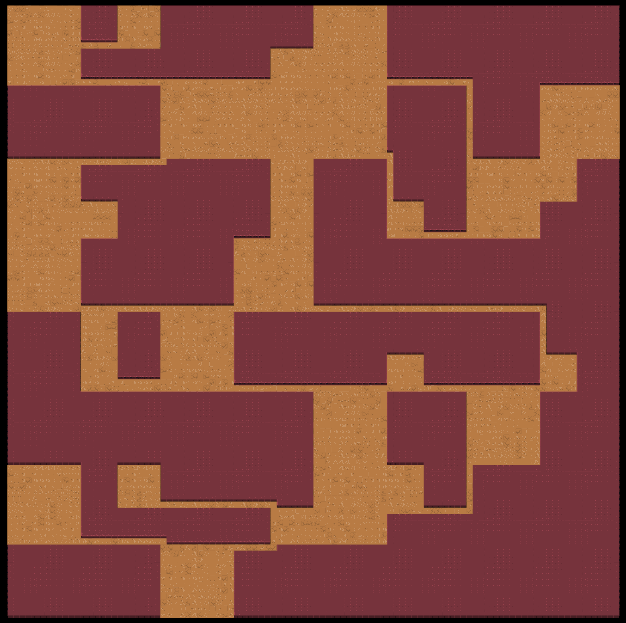
\includegraphics[width=.8\linewidth]{../images/pcg_quadtree/pcg1.png}
  \label{fig:sfig1}
\end{subfigure}%
\begin{subfigure}{.5\textwidth}
  \centering
  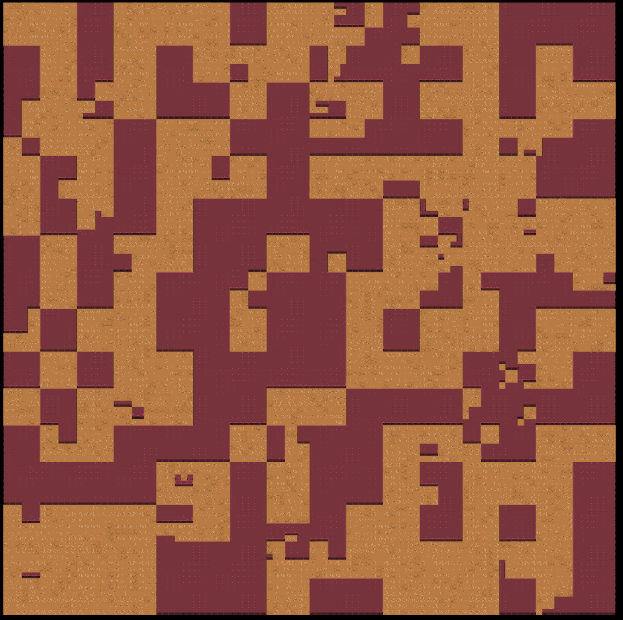
\includegraphics[width=.8\linewidth]{../images/pcg_quadtree/pcg2.png}
  \label{fig:sfig2}
\end{subfigure}
\begin{subfigure}{.5\textwidth}
  \centering
  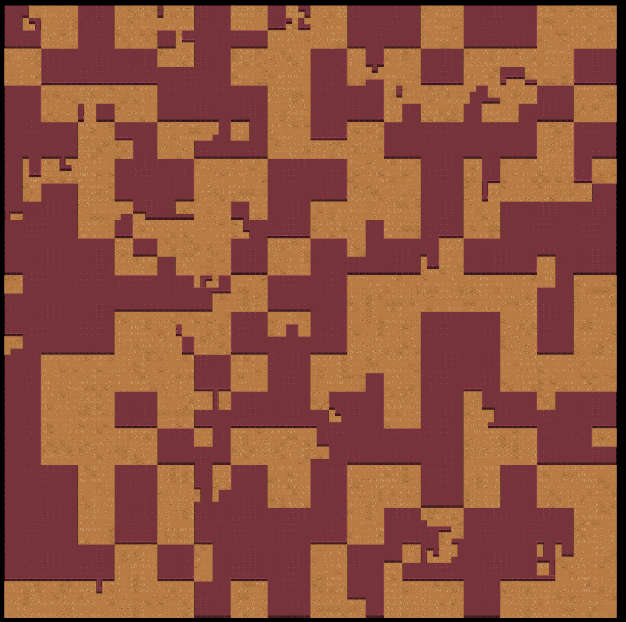
\includegraphics[width=.8\linewidth]{../images/pcg_quadtree/pcg3.png}
  \label{fig:sfig1}
\end{subfigure}%
\begin{subfigure}{.5\textwidth}
  \centering
  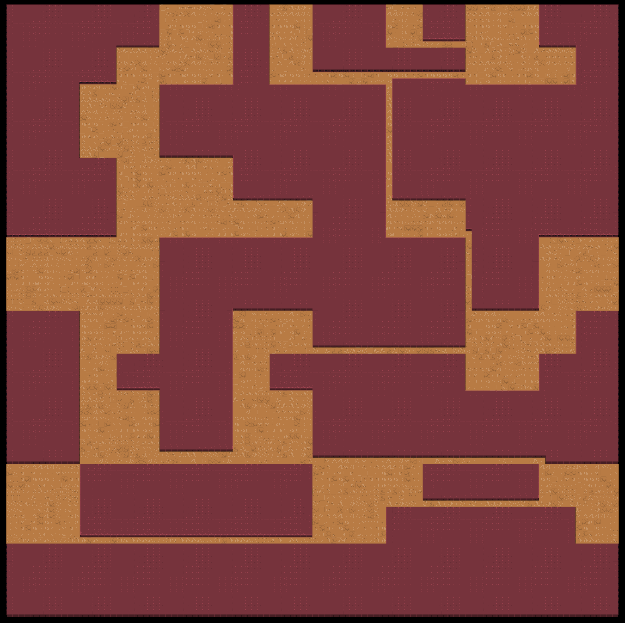
\includegraphics[width=.8\linewidth]{../images/pcg_quadtree/pcg4.png}
  \label{fig:sfig2}
\end{subfigure}
\begin{subfigure}{.5\textwidth}
  \centering
  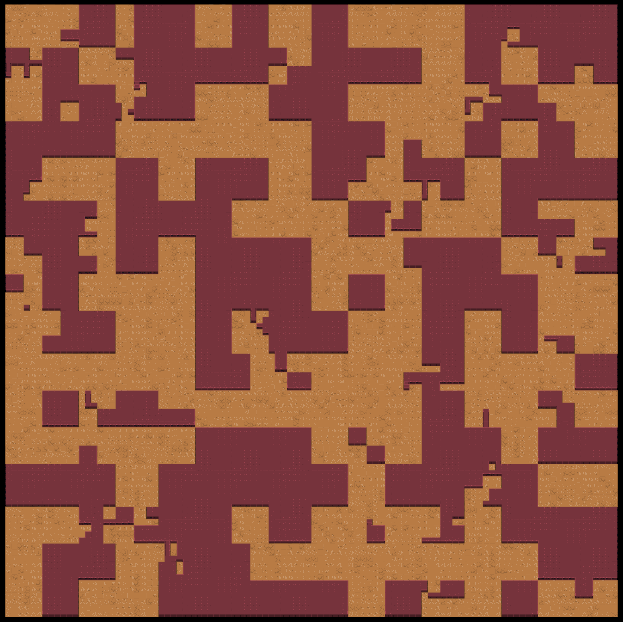
\includegraphics[width=.8\linewidth]{../images/pcg_quadtree/pcg5.png}
  \label{fig:sfig1}
\end{subfigure}%
\begin{subfigure}{.5\textwidth}
  \centering
  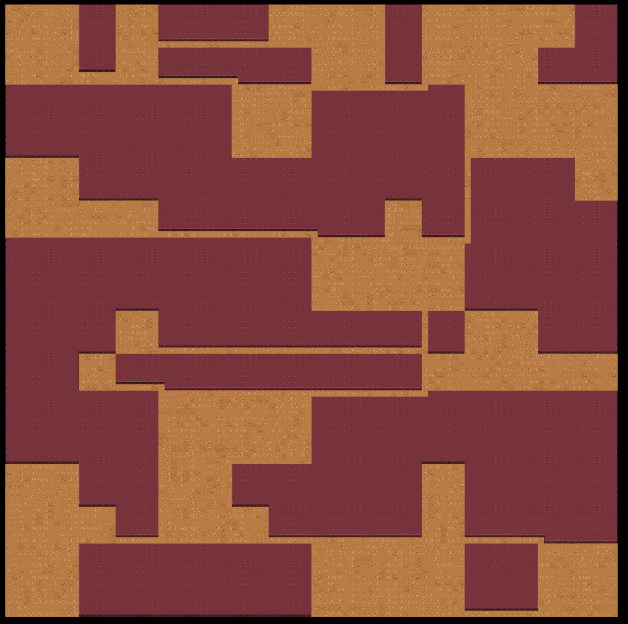
\includegraphics[width=.8\linewidth]{../images/pcg_quadtree/pcg6.png}
  \label{fig:sfig2}
\end{subfigure}
\caption{Μερικά από τα επίπεδα που δημιουργήθηκαν από το σύστημα του PCG, με split possibility=0,3 και room possibility=0,6.}
\label{fig:fig}
\end{figure}


\section{Διάνοιξη Διαδρόμων}
Η διάνοιξη διαδρόμων εφαρμόζετε μετά την δημιουργία δωματίων για να εξασφαλίσει ότι θα υπάρχει κάποιο μονοπάτι πρόσβασης από και προς όλα τα δωμάτια. Η εφαρμογή ενός αλγορίθμου διάνοιξης διαδρόμων εξασφαλίζει ότι το επίπεδο που δημιουργήθηκε είναι \textit{playable} με βάση την πρόσβαση στα δωμάτια από οποιαδήποτε ανοιχτό σημείο του επιπέδου.

\subsection{Εύρεση δωματίων}
\par
Για την εφαρμογή της διάνοιξης, απαιτείται πρώτα να γνωρίζουμε και να έχουμε αποθηκευμένα τα στοιχεία του κάθε δωματίου. Επομένως πρώτο βήμα του αλγορίθμου διάνοιξης είναι η εύρεση όλων των ξεχωριστών δωματίων που υπάρχουν σε ένα επίπεδο. Ως δωμάτιο θεωρούμε έναν ανοιχτό χώρο στον οποίο ο παίκτης μπορεί να περιηγηθεί με οριζόντιες και κάθετες κινήσεις. Οι διαγώνιες κινήσεις θεωρούνται συνδυασμός των κάθετων και οριζοντίων σε αυτή την εφαρμογή.
\par
O αλγόριθμος εύρεσης δωματίων ελέγχει όλα τα tiles του επιπέδου σειριακά από κάτω αριστερά προς δεξιά και πάνω. Μόλις βρει ένα \textit{tile} το οποίο είναι είδους δωματίου ξεκινάει ο αλγόριθμος υπολογισμού του δωματίου. 
\begin{enumerate}
\item Δημιουργείται ένα νέο αντικείμενο \textit{Room} στο οποίο θα αποθηκευτούν όλα τα \textit{tiles} που ανήκουν σε αυτό το δωμάτιο.
\item Το στοιχείο που βρέθηκε πρώτο προστίθεται σε μια δομή αναζήτησης είδους ουρά(\textit{queue}).
\item Ξεκινάει μια επανάληψη η οποία διαρκεί όσο η ουρά αναζήτησης περιέχει στοιχεία. Σε κάθε βήμα της επανάληψης:
\item Αφαιρείται το πρώτο στοιχείο της ουράς και εάν είναι είδους δωματίου προστίθεται στο Room.
\item Όλα τα γειτονικά στοιχεία του συγκεκριμένου στοιχείου προστίθενται στην ουρά. Γειτονικά στοιχεία ορίζονται ως τα οριζόντια και κάθετα στοιχεία που βρίσκονται δίπλα στο επιλεγμένο στοιχείο.
\item Μόλις η ουρά αναζήτησης αδειάσει, το αντικείμενο Room που δημιουργήθηκε προστίθεται σε μια λίστα που αποθηκεύει όλα τα δωμάτια του επιπέδου.
\end{enumerate}
Για την αποφυγή \textit{duplicates} δημιουργείται και μια δομή \textit{HashMap} η οποία αποθηκεύει κάθε στοιχείο που έχει ελεγθεί από τον αλγόριθμο υπολογισμού δωματίου.

\begin{figure}[H]
\begin{subfigure}{.5\textwidth}
  \centering
  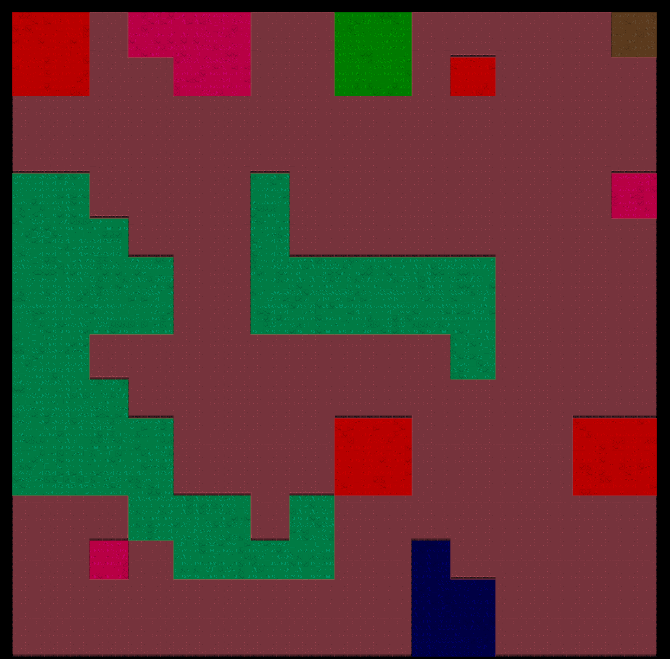
\includegraphics[width=.8\linewidth]{../images/colored_rooms/1.png}
  \label{fig:sfig1}
\end{subfigure}%
\begin{subfigure}{.5\textwidth}
  \centering
  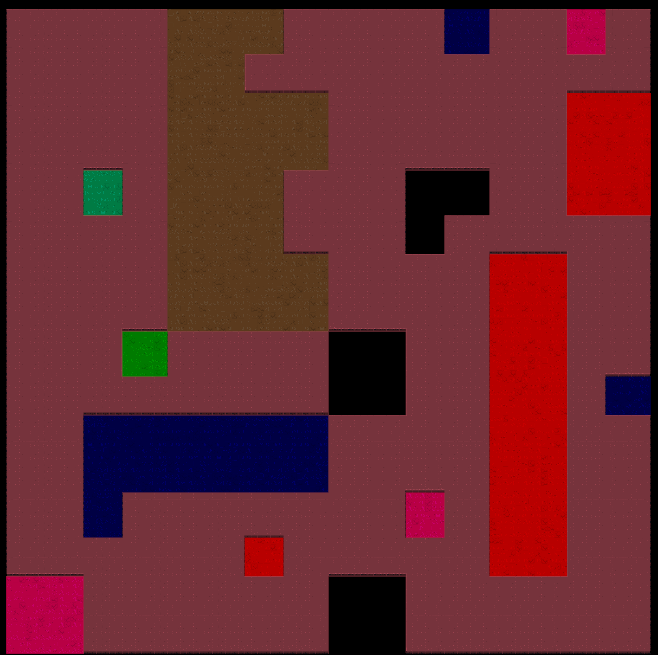
\includegraphics[width=.8\linewidth]{../images/colored_rooms/2.png}
  \label{fig:sfig2}
\end{subfigure}
\begin{subfigure}{.5\textwidth}
  \centering
  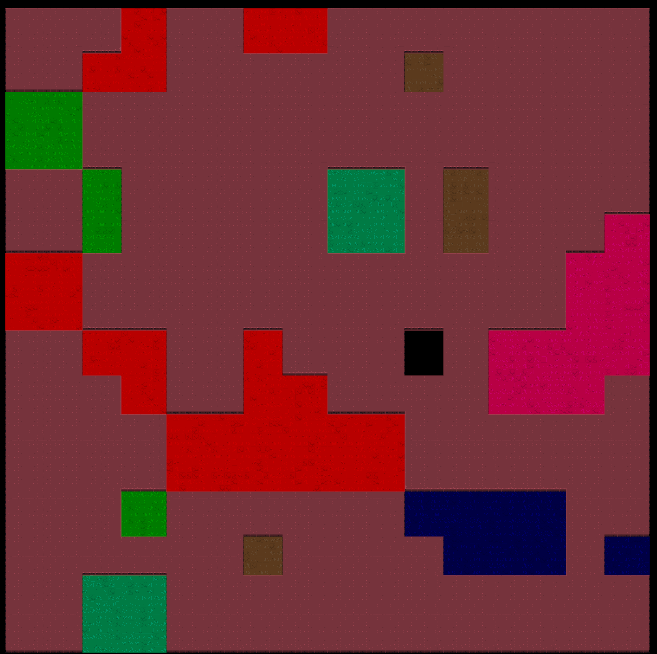
\includegraphics[width=.8\linewidth]{../images/colored_rooms/3.png}
  \label{fig:sfig1}
\end{subfigure}%
\begin{subfigure}{.5\textwidth}
  \centering
  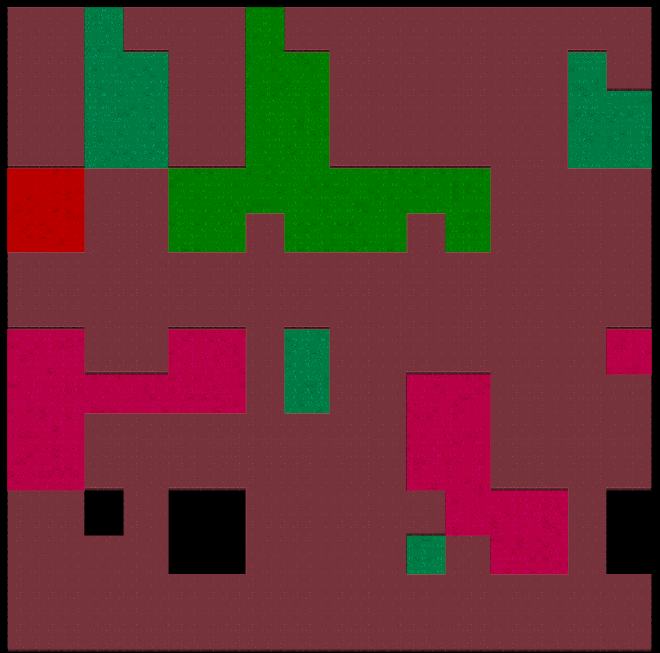
\includegraphics[width=.8\linewidth]{../images/colored_rooms/4.png}
  \label{fig:sfig2}
\end{subfigure}
\caption{Σε αυτές τις εικόνες φαίνονται χρωματισμένα τα δωμάτια που έχει εντοπίσει και αποθηκεύσει ο αλγόριθμος εύρεσης δωματίων.}
\label{fig:fig}
\end{figure} 



\subsection{Διάνοιξη Διαδρόμων}
\par
Μόλις ολοκληρωθεί ο αλγόριθμος εύρεσης δωματίων, έχουμε αποθηκευμένα τα δωμάτια σε μια λίστα με το κάθε δωμάτιο να περιλαμβάνει τα \textit{tiles} που το αποτελούν. Το κάθε \textit{tile} έχει ως πληροφορίες τις συντεταγμένες του μέσα στο επίπεδο και το είδος του. Ο αλγόριθμος διάνοιξης διαδρόμων ξεκινάει με το πρώτο δωμάτιο της λίστα ως αρχικό δωμάτιο και το δεύτερο δωμάτιο ως τελικό δωμάτιο. Υπολογίζει ποιά στοιχεία των δύο δωματίων έχουν την μικρότερη μεταξύ τους απόσταση, με βάση την απόσταση \textit{Manhattan} και στη συνέχεια ανοίγει έναν διάδρομο μεταξύ αυτών των δύο στοιχείων. Τα δύο δωμάτια είναι πλέον ενωμένα με έναν διάδρομο. Ο αλγόριθμος συνεχίζει επιλέγοντας ως αρχικό δωμάτιο το δεύτερο δωμάτιο της λίστας και ως τελικό δωμάτιο το τρίτο δωμάτιο της λίστας μέχρι να συνδέσει όλα τα δωμάτια του επιπέδου με τον παραπάνω τρόπο.
\par
H διάνοιξη διαδρόμου μεταξύ δύο σημείων γίνετε ξεκινώντας από το αρχικό σημείο, το οποίο είναι αυτό με τη μικρότερη συντεταγμένη \textit{x}, διασχίζει τα στοιχεία μέχρι να φτάσει στο σημείο που έχει ίδια συντεταγμένη \textit{x} με το τελικό σημείο. Κατά την διάσχιση αλλάζει το είδος των στοιχείων από τοίχο σε δωμάτιο. Το ίδιο επαναλαμβάνετε και για την συντεταγμένη \textit{y} από το στοιχείο στο οποίο σταμάτησε ο αλγόριθμος για την συντεταγμένη \textit{x}.

\begin{figure}[H]
\begin{subfigure}{.5\textwidth}
  \centering
  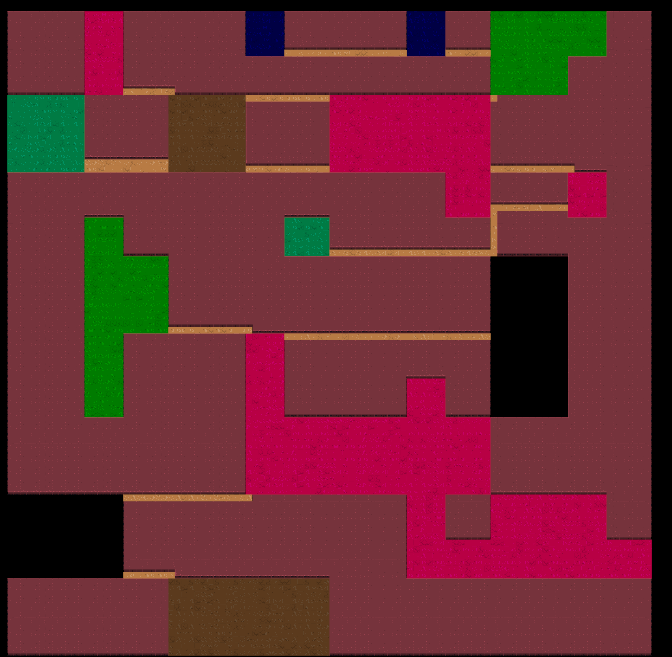
\includegraphics[width=.8\linewidth]{../images/colored_rooms/c_1.png}
  \label{fig:sfig1}
\end{subfigure}%
\begin{subfigure}{.5\textwidth}
  \centering
  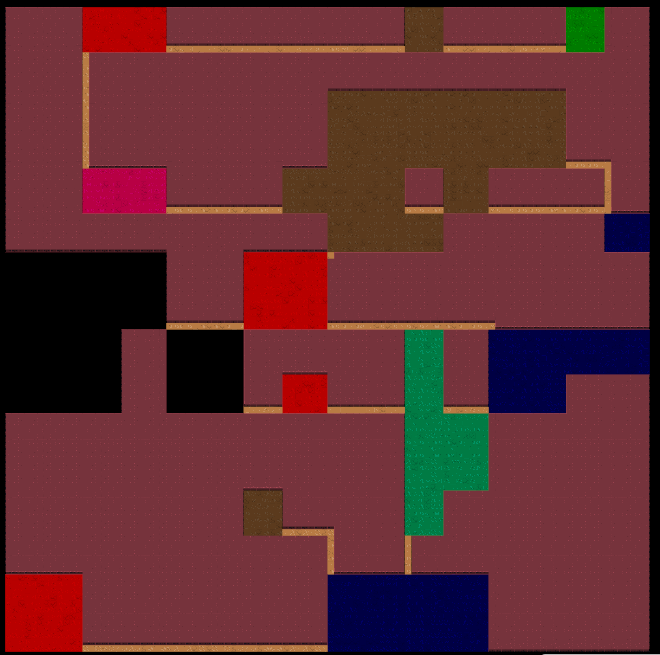
\includegraphics[width=.8\linewidth]{../images/colored_rooms/c_2.png}
  \label{fig:sfig2}
\end{subfigure}
\begin{subfigure}{.5\textwidth}
  \centering
  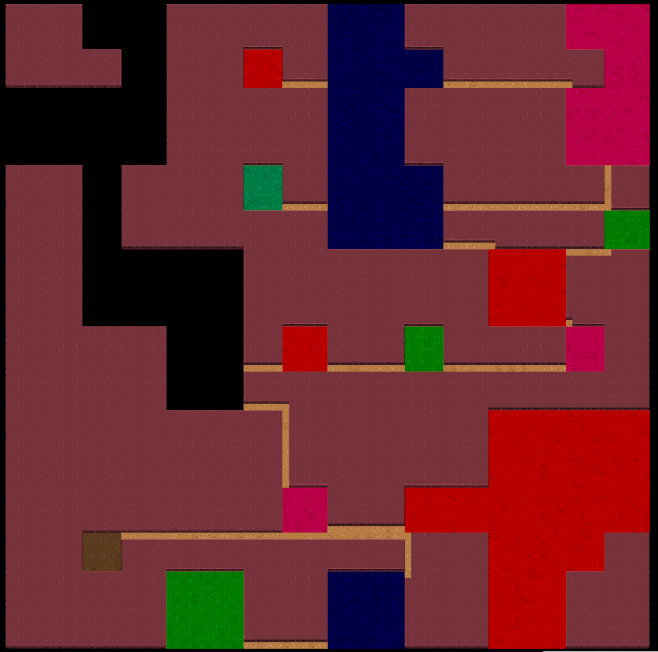
\includegraphics[width=.8\linewidth]{../images/colored_rooms/c_3.png}
  \label{fig:sfig1}
\end{subfigure}%
\begin{subfigure}{.5\textwidth}
  \centering
  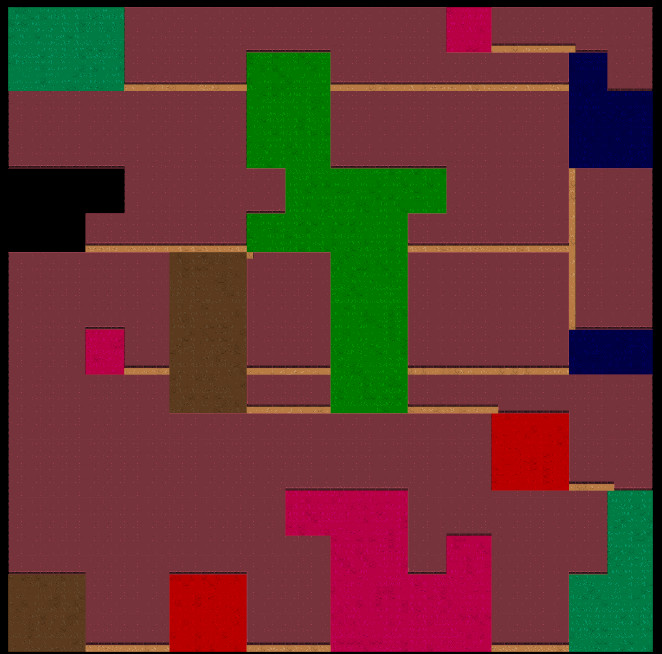
\includegraphics[width=.8\linewidth]{../images/colored_rooms/c_4.png}
  \label{fig:sfig2}
\end{subfigure}
\caption{Παραδείγματα επιπέδων μετά την διάνοιξη διαδρόμων}
\label{fig:fig}
\end{figure}











